\documentclass[sigconf]{acmart}
\usepackage{graphicx}

\usepackage{graphicx}
\usepackage{hyperref}
\usepackage{todonotes}

\usepackage{endfloat}
\renewcommand{\efloatseparator}{\mbox{}} % no new page between figures

\usepackage{booktabs} % For formal tables

\settopmatter{printacmref=false} % Removes citation information below abstract
\renewcommand\footnotetextcopyrightpermission[1]{} % removes footnote with conference information in first column
\pagestyle{plain} % removes running headers

\newcommand{\TODO}[1]{\todo[inline]{#1}}
\begin{document}
\title{Big Data and League of Legends}


\author{Junjie Lu}
% \orcid{1234-5678-9012}
\affiliation{%
  \institution{Indiana University Bloomington}
  \streetaddress{3322 John Hinkle Place}
  \city{Bloomington} 
  \state{Indiana} 
  \postcode{47408}
}
\email{junjlu@iu.edu}


% The default list of authors is too long for headers}
% \renewcommand{\shortauthors}{G. v. Laszewski}


\begin{abstract}
League of Legends is the most popular MOBA online game in these years. There are millions of players all over the world. And big data about League of Legends is also deserved to be researched. The data could tell us many things we do not know. We could know usage of champions by learning weekly free champion rotation. Then getting some information of a part of income of Riot Game company. Also we could learning some advanced information of this game by researching win rate and something else. These could help players getting a better performance in the game. Further more, we can also try to figure out which side would win the game before it ends. All this is from big data analysis. 
\end{abstract}

\keywords{I523, HID214, Big Data, League of Legends, Win rate, Income}


\maketitle



\section{Introduction}
Computer games become more and more popular in these years. Children could play different single games on computer ten years ago. Different kinds of online games were produced in the past decade. And they have a really large market now. In 2016, market of video game all over the world is more than 111 billion.\cite{bbb} MOBA game (Multiplayer Online Battle Arena) occupies the most players because of its flexibility and uncertainty. The most successful MOBA game is League of Legend. In America, it has more than 30 million players and ten times of it in worldwide. That is an amazing number meaning a large succeed. Player could pick a champion before the game and fight with the champion he picked as a team with five persons. There are 137 existing champions and the number is still growing. Different champions play different role in their team with their own capability. It is interesting playing different champions. Players must pay for champions so that they could use them. Riot game, the producer of League of Legends sets free 10 champions every week to give players better playing experience. If player likes these champions, they could purchase them so that they can use them anytime. Further more they can also buy some skins which can give champions better appearance. These could bring Riot Game much income. We could analyze the influence of free champions on income and some other fields.
\section{Data Analysis for incoming}
We could get much data on LoLDB website. It can tell you much about champions such as win rate, pick rate and so on. Before analysis, we should know there are different tiers in League of Legends. It can tell people how intelligent a player is. We just pick from normal to Diamond. According to the data, we could get the usage of a champion just name it AB as follow:\\
\begin{equation}
    U_t=100*\frac{M_t}{\sum_{c=1}^C\frac{W_t}{5}}
\end{equation}
In this equation, $M_t$ is the number of match in which champion AB being selected in tier $t$ on one day. $W_t$ means total winners in tier $t$. \cite{ccc} The usage score roughly translates to the percent of games in which a champion appears and allows for an increased score when popular champions appear on both teams.\cite{ddd} \\

According to Figure 1, the usage of free champions is absolutely increased especially in lower tiers. And the usage of champions free on previous week is still higher than champions who are not free recently. We can get that amount of players payed for their beloved champions after using them freely. \\

As the data from Figure 2, we can get the probability of players who bought champions after playing with free champion rotation. And we can get:\\
\begin{equation}
    I=\sum_{c=1}^{10}\sum_{t=1}^6a*U*p_c
\end{equation}
$I$ is the income by selling champions. $a$ is a constant of price of champion. $p_c$ is the probability of purchasing champions. So we can get income of selling champions of Riot Game approximately with this equation. \\
Further more, skin can also bring income for Riot Game. As a survey in China about if players are forward to purchasing a skin for champion he love. It can not only bring a better appearance for the champions, but also some confidence when fighting with the champion. More than 30\% users are willing to buy skins according to the survey in Figure 3. One champion could have different kinds of skins with different prices. \\

\begin{equation}
    I_s=\sum_{c=1}^{10}\sum_{t=1}^6b*U*p_s
\end{equation}
$b$ is a constant for value of skins and $p_s$ is the percentage of players buying skins. We can get $I$ and $I_S$ as incoming of Riot Game by selling champions and skins from data analysis.
\section{Prediction for patch}
All games need balance. There are more than 130 champions in League of Legends and they all have their own abilities, playing different roles. Designer should give equal ability to get some usage of players. But it is a really difficult task. When we strength champion A and its usage increases, that must means usage of another champion decreased. Also if champion C always has a wonderful performance when he faces champion D, the usage of champion D won't be high if usage of champion C is high. To deal with this situation, designers must fix features of champions patch next patch. They not only fix bug of the game, but also buff or debuff champions  in turn to make sure they could got enough picked. In this case, designer would only adjust several champions in each patch. With more than two year observation, we found that designers prefer to adjust champions whom has higher win rate. A higher win rate means players prefer to pick them to have a easy win. This limits usage of other champions. Hence designer have to make some adjustment on the champion, such as turn down the damage it can make or increasing cool down time of skills. Designers always take this way to keep balance between champions. For example, in Patch 6.13, champion Graves has a out of power win rate 57\%. This is much higher than the average and means that Graves occupies the most usage. Designers strengthened champion Kindred by increasing its armor so that it can beat Graves in late game. And increased damage of champion Nidalee encouraging it beats Graves in early games. Then we can see the win rate of these three champions are approximately equal in next patch. That is what they want. With this thought, we could use the big data of win rate and some else to predict something of patch. For instance, champion Galio has a pretty good performance in matches with a win rate of 54\%. So I think champion Malzahar and Vayne will get buffed in next patch to limit win rate of Galio. There is something more what we have to consider is the impact of new champions. Most of new champions, will stand on its usage peek for one week or two, and cool down after it is free week. Then it will become as other champions. Some thing different is champion Yasuo, for unknown reason, its usage is high stably. No matter how designer weaken it, there are still millions of players loving it and fighting with it. People have to admit it is the most popular champion they have seen. What is more we have to pay attention is champion reworking. For instance, champion Sion got rework in patch 4.18 and we can see a tremendous increase in usage in October 2014  The usage stabilizes quickly overtime, and it remains mostly unaffected during his free week because many players already own Sion (due to his age) and inexpensiveness. \cite{aaa}
\section{Judge toxic behavior}
The game has its own report system, players could report others who has toxic behavior. But it is hard to say who is really toxic if two players report each other. Big data helps a lot here. The data KDA(Kill-Death-Assist) is essential in this part. \\
\begin{equation}
    KDA=\frac{Kill + Assist}{Death}
\end{equation}
Players who has toxic behavior always has a negative attitude to the match. In this case, the value of KDA is always pretty small. Number of killing minions $cs$ could also make some contribution in this part. \\
\begin{equation}
    T=\frac{KDA*cs}{R}
\end{equation}
Number $R$ is time of reported gotten from teammates in one game. In this case, when we got some report form players, we could use big data to judge value $T$ to get conclusion of people who is really toxic one. The player is toxic when value of $T$ is pretty low. System could give toxic players some punishment and prevent from give punishment to wrong people. 
\section{Predict result of matches for further work}
These days the world championship is in China. 16 teams are fighting for the final championship. The competition is a little different from normal games. Each side could ban 5 champions in one match. And one champion could not pick twice on one side or two. There are many strategy on ban and pick, and this is coaches' job. How to pick 5 good champions after banning 10 champions totally helping winning the match. Coaches need to refer big data, not only win rate of every champion, but also win rate of champions when players in his team playing them. What is more, data from OP website could provide more data in detail such as win rate of champion A when facing champion B. Above all it needs a complex model to predict the result of a match. So it is further work. 
\section{Conclusion}
Big data could help us to analyze much useful information. We could know how much Riot Game earn by selling champions and skins. And having a judgement to the patch. Players could practice champions would get strengthen in advance. It could help them get a higher win rate before everyone got this. And people may get result prediction of a match before it begins in the future. 
\begin{acks}

The author would like to thank Professor Gregor von Laszewski and all TAs for providing the resource, tutorials and other related materials to write this paper.

\end{acks}

\bibliographystyle{ACM-Reference-Format}
\bibliography{report}
\begin{figure}{htp}
\centering
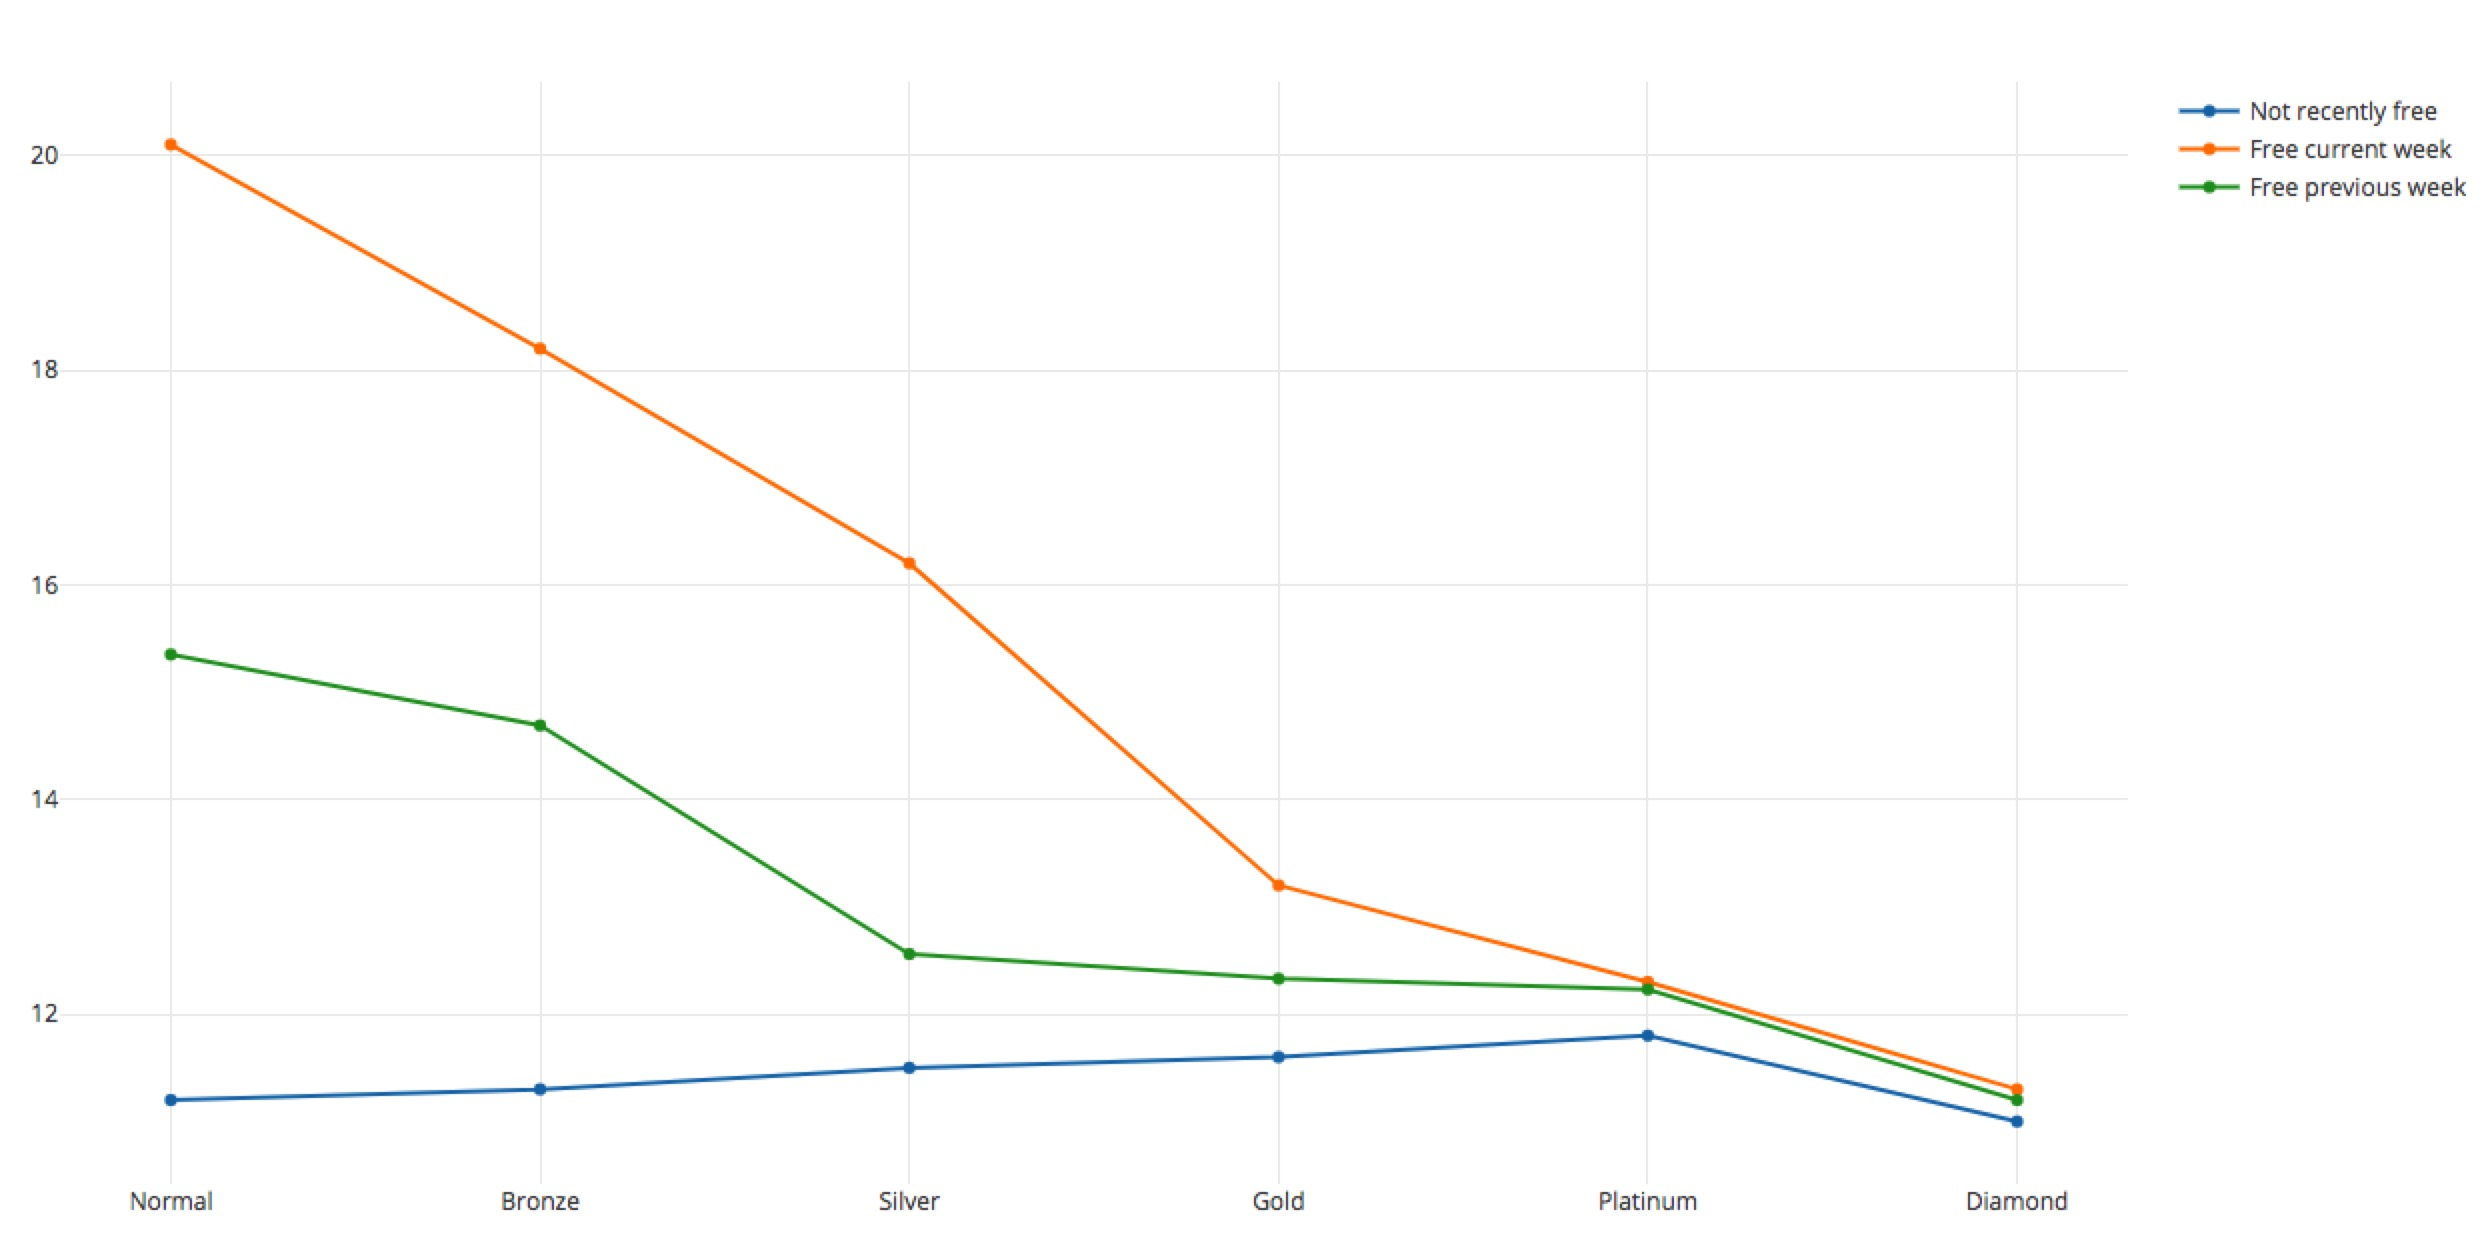
\includegraphics[width=1.0\textwidth]{images/WechatIMG112.jpeg}
\caption{Usage of free champion}
\label{Figure 1}
\end{figure}
\begin{figure}{htp}
\centering
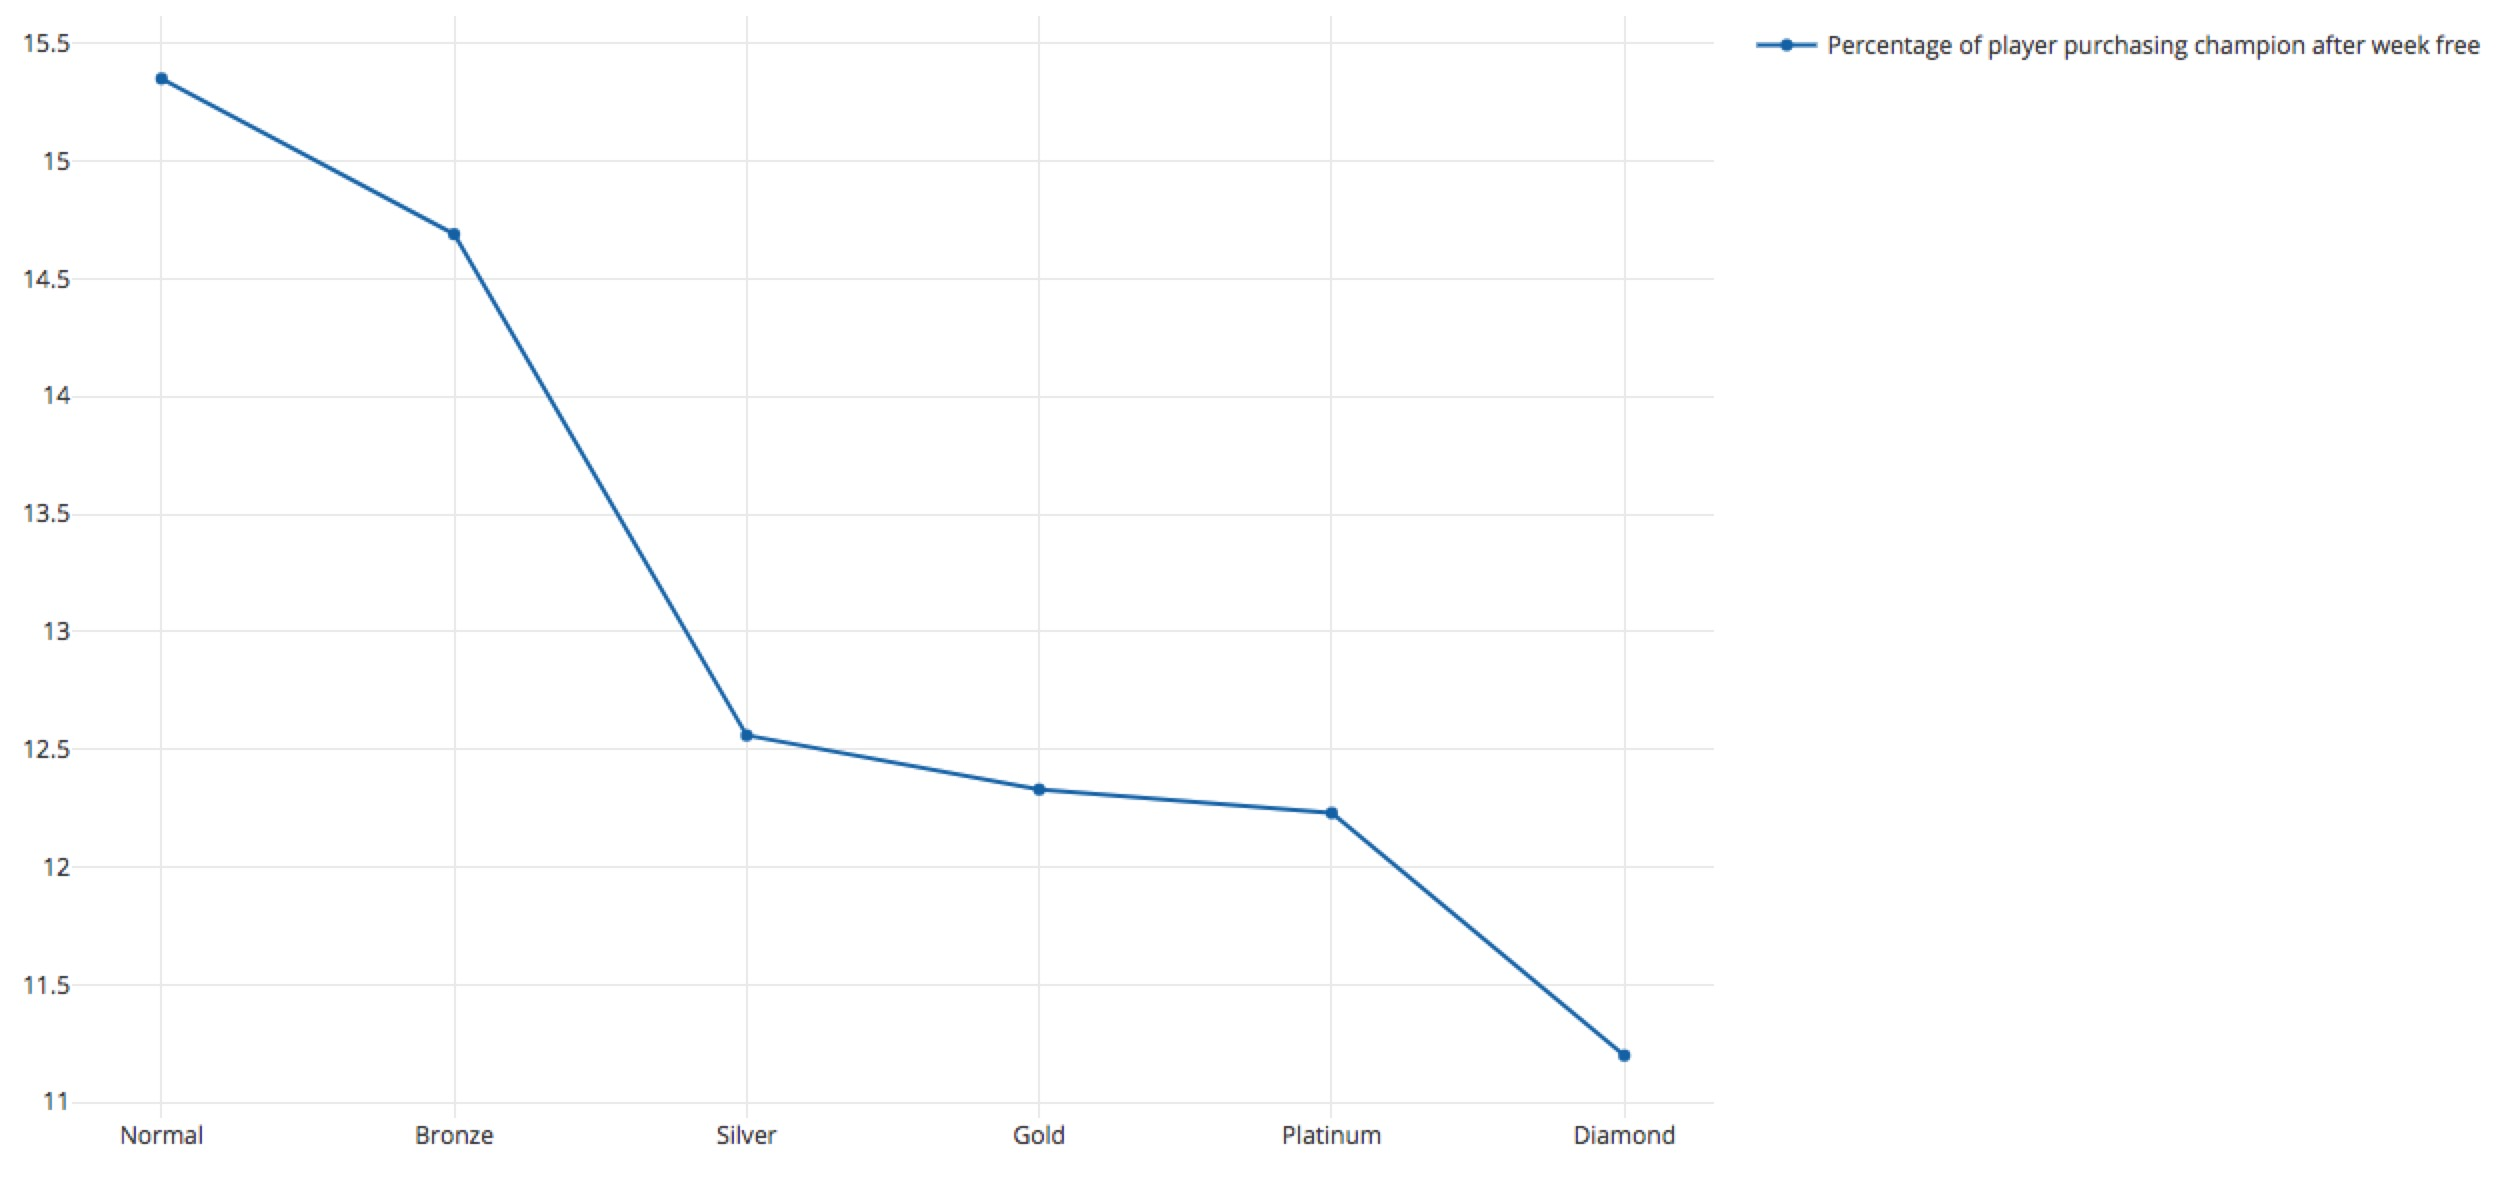
\includegraphics[width=1.0\textwidth]{images/WechatIMG114.jpeg}
\caption{Probability of purchasing champion}
\label{Figure 2}
\end{figure}
\begin{figure}{htp}
\centering
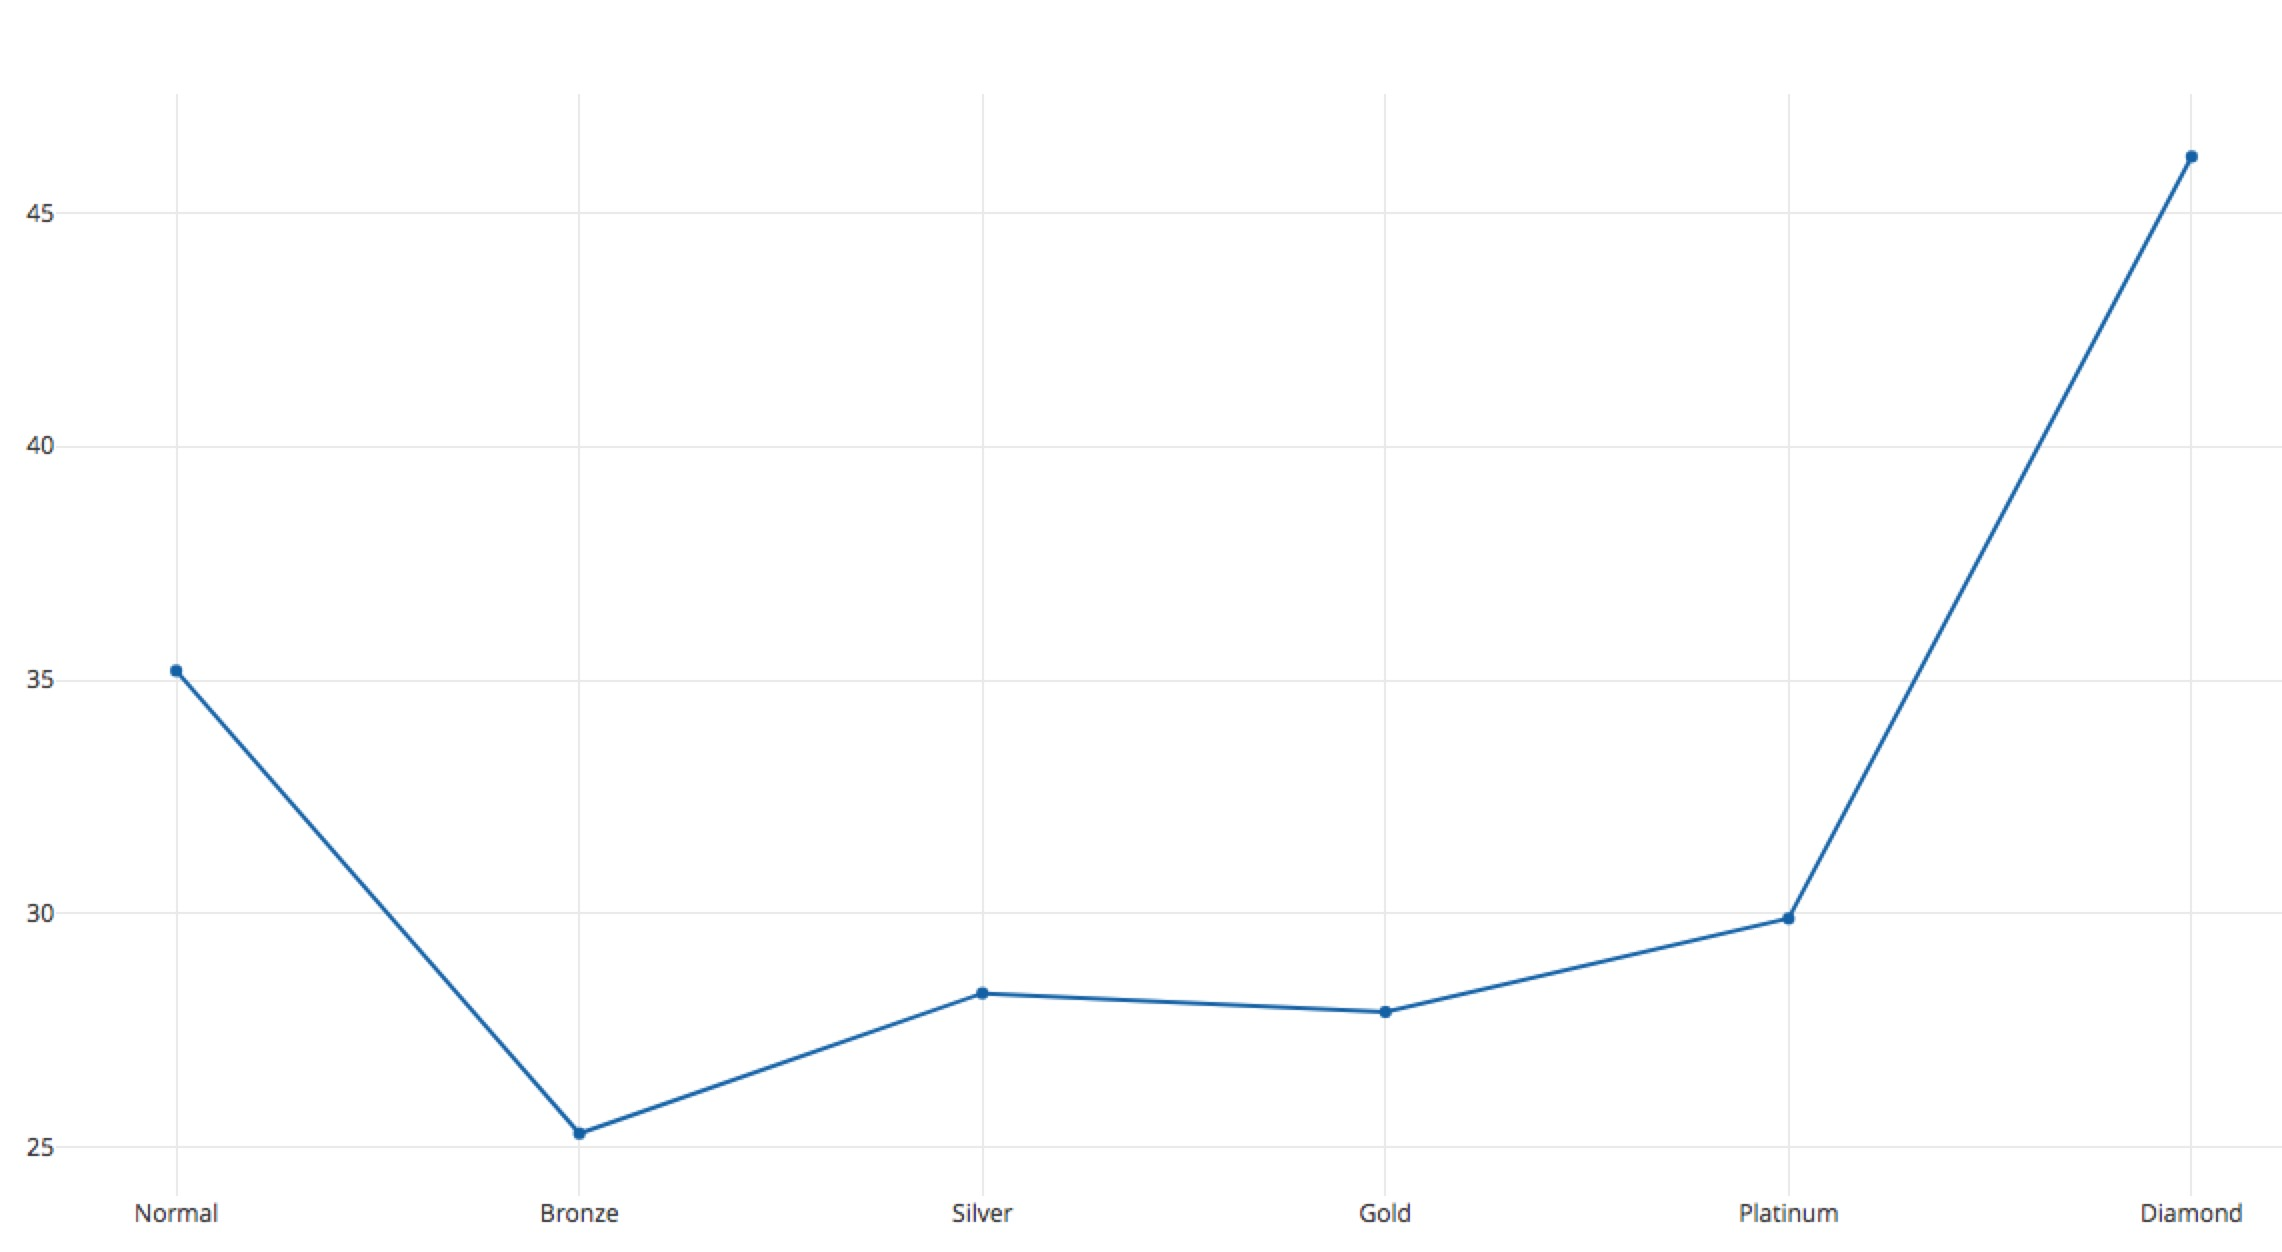
\includegraphics[width=1.0\textwidth]{images/WechatIMG115.jpeg}
\caption{Percentage of players willing to buy skins}
\label{Figure 3}
\end{figure}
% \section{Issues}

\DONE{Example of done item: Once you fix an item, change TODO to DONE}

\subsection{Assignment Submission Issues}

    \TODO{Do not make changes to your paper during grading, when your repository should be frozen.}

\subsection{Uncaught Bibliography Errors}

    \TODO{Missing bibliography file generated by JabRef}
    \TODO{Bibtex labels cannot have any spaces, \_ or \& in it}
    \TODO{Citations in text showing as [?]: this means either your report.bib is not up-to-date or there is a spelling error in the label of the item you want to cite, either in report.bib or in report.tex}

\subsection{Formatting}

    \TODO{Incorrect number of keywords or HID and i523 not included in the keywords}
    \TODO{Other formatting issues}

\subsection{Writing Errors}

    \TODO{Errors in title, e.g. capitalization}
    \TODO{Spelling errors}
    \TODO{Are you using {\em a} and {\em the} properly?}
    \TODO{Do not use phrases such as {\em shown in the Figure below}. Instead, use {\em as shown in Figure 3}, when referring to the 3rd figure}
    \TODO{Do not use the word {\em I} instead use {\em we} even if you are the sole author}
    \TODO{Do not use the phrase {\em In this paper/report we show} instead use {\em We show}. It is not important if this is a paper or a report and does not need to be mentioned}
    \TODO{If you want to say {\em and} do not use {\em \&} but use the word {\em and}}
    \TODO{Use a space after . , : }
    \TODO{When using a section command, the section title is not written in all-caps as format does this for you}\begin{verbatim}\section{Introduction} and NOT \section{INTRODUCTION} \end{verbatim}

\subsection{Citation Issues and Plagiarism}

    \TODO{It is your responsibility to make sure no plagiarism occurs. The instructions and resources were given in the class}
    \TODO{Claims made without citations provided}
    \TODO{Need to paraphrase long quotations (whole sentences or longer)}
    \TODO{Need to quote directly cited material}

\subsection{Character Errors}

    \TODO{Erroneous use of quotation marks, i.e. use ``quotes'' , instead of " "}
    \TODO{To emphasize a word, use {\em emphasize} and not ``quote''}
    \TODO{When using the characters \& \# \% \_  put a backslash before them so that they show up correctly}
    \TODO{Pasting and copying from the Web often results in non-ASCII characters to be used in your text, please remove them and replace accordingly. This is the case for quotes, dashes and all the other special characters.}
    \TODO{If you see a figure and not a figure in text you copied from a text that has the fi combined as a single character}

\subsection{Structural Issues}

    \TODO{Acknowledgement section missing}
    \TODO{Incorrect README file}
    \TODO{In case of a class and if you do a multi-author paper, you need to add an appendix describing who did what in the paper}
    \TODO{The paper has less than 2 pages of text, i.e. excluding images, tables and figures}
    \TODO{The paper has more than 6 pages of text, i.e. excluding images, tables and figures}
    \TODO{Do not artificially inflate your paper if you are below the page limit}

\subsection{Details about the Figures and Tables}

    \TODO{Capitalization errors in referring to captions, e.g. Figure 1, Table 2}
    \TODO{Do use {\em label} and {\em ref} to automatically create figure numbers}
    \TODO{Wrong placement of figure caption. They should be on the bottom of the figure}
    \TODO{Wrong placement of table caption. They should be on the top of the table}
    \TODO{Images submitted incorrectly. They should be in native format, e.g. .graffle, .pptx, .png, .jpg}
    \TODO{Do not submit eps images. Instead, convert them to PDF}

    \TODO{The image files must be in a single directory named "images"}
    \TODO{In case there is a powerpoint in the submission, the image must be exported as PDF}
    \TODO{Make the figures large enough so we can read the details. If needed make the figure over two columns}
    \TODO{Do not worry about the figure placement if they are at a different location than you think. Figures are allowed to float. For this class, you should place all figures at the end of the report.}
    \TODO{In case you copied a figure from another paper you need to ask for copyright permission. In case of a class paper, you must include a reference to the original in the caption}
    \TODO{Remove any figure that is not referred to explicitly in the text (As shown in Figure ..)}
    \TODO{Do not use textwidth as a parameter for includegraphics}
    \TODO{Figures should be reasonably sized and often you just need to
  add columnwidth} e.g. \begin{verbatim}/includegraphics[width=\columnwidth]{images/myimage.pdf}\end{verbatim}

re

\end{document}